\documentclass[a4paper,12pt]{report}            % [forma A4, taille police] {Type}
    \usepackage[utf8]{inputenc}                
    \usepackage[T1]{fontenc}                        % Codage des fontes TeX
    \usepackage[francais]{babel}
    \usepackage{graphicx}
    \usepackage{wrapfig}
    \usepackage{fancyhdr}
    \usepackage{xcolor}
    \usepackage{hyperref}
    \usepackage{listings}
    \usepackage{fullpage}
    \usepackage{eso-pic}
    \usepackage{titlesec}
    \titleformat{\chapter}[hang]{\bf\huge}{\thechapter}{2pc}{}
    \lstset {numbers=left ,stepnumber=1,firstnumber=0,numberfirstline=true}
    \hypersetup{
        bookmarks=true,         % show bookmarks bar?
        unicode=false,          % non-Latin characters in Acrobat’s bookmarks
        pdftoolbar=true,        % show Acrobat’s toolbar?
        pdfmenubar=true,        % show Acrobat’s menu?
        pdffitwindow=false,     % window fit to page when opened
        pdfstartview={FitH},    % fits the width of the page to the window
        pdftitle={My title},    % title
        pdfauthor={Author},     % author
        pdfsubject={Subject},   % subject of the document
        pdfcreator={Creator},   % creator of the document
        pdfproducer={Producer}, % producer of the document
        pdfkeywords={keyword1, key2, key3}, % list of keywords
        pdfnewwindow=true,      % links in new PDF window
        colorlinks=true,       % false: boxed links; true: colored links
        linkcolor=black,          % color of internal links (change box color with linkbordercolor)
        citecolor=green,        % color of links to bibliography
        filecolor=magenta,      % color of file links
        urlcolor=blue           % color of external links
    }
    
    \author{Samuel HUET \& Thomas COUTANT}
    \title{\huge{\textbf{L'Amplificateur}}}
    
    \begin{document}
\maketitle
\renewcommand{\contentsname}{SOMMAIRE} % Dans le corps du document,avant la commande \tableofcontents.
\tableofcontents

\chapter{Petits signaux}
\addcontentsline{toc}{chapter}{Petits signaux}

\section{Pertes}

Afin de déterminer le gain de l'amplificateur fournis, nous devons le brancher 
à un oscillateur à son entré, puis à un analyseur de spectre de l'autre. Ainsi, 
la différence entre l'amplitude (à la fréquence donné) en entré et en sortie nous 
donnera son gain. 

Cependant, certaines précautions sont à prendre : Afin d'éliminer les pertes du aux cables, 
nous devons relier l'oscillateur dirrectement à l'analyseur. Et enfin, afin d'éviter
tout risque d'endomager ou d'écréter le signal en entré de l'analyseur, nous rajouterons
un aténuateur à son entré.

\begin{center}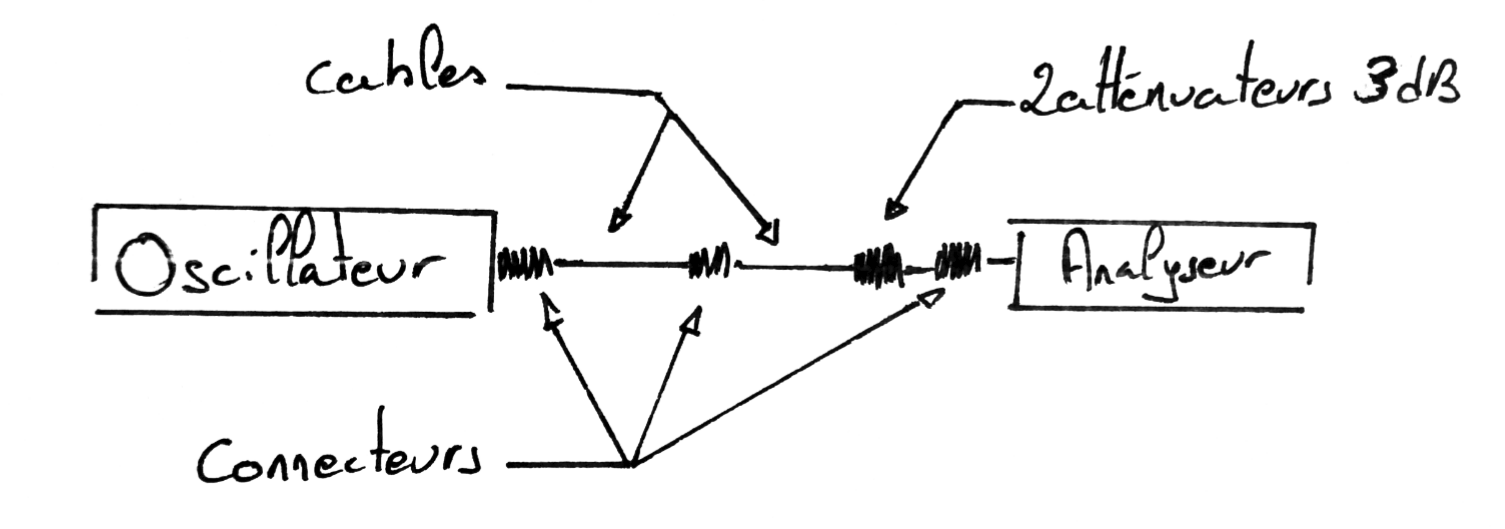
\includegraphics[scale = 0.25]{pic/perte_cables.png}\\ \end{center}

Le résultat que nous trouvons dépend de la fréquence, nous avons alors tracé un graphique
montrant les pertes dus aux cables, connecteurs et atténuateurs en fonction de la fréquence.

\begin{center}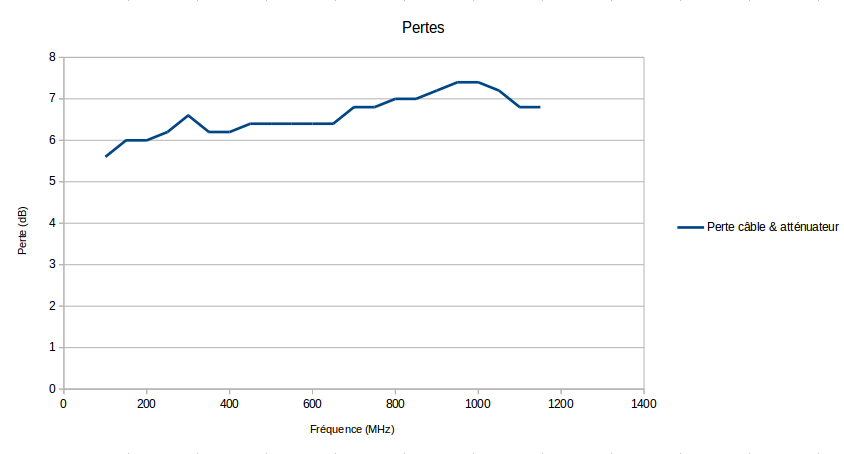
\includegraphics[scale = 0.4]{pic/perte_graph.png}\\ \end{center}

Nous prendrons donc soins d'ajouter les pertes en fonction de la fréquences à chaque mesure.
Maintenant que nous avons déterminé les pertes, nous pouvons nous atteler à notre première mesure !


\section{Gain}

Afin de procéder à la mesure du gain en fonction de la fréquence, utilisons ce cablage ci-dessous :

\begin{center}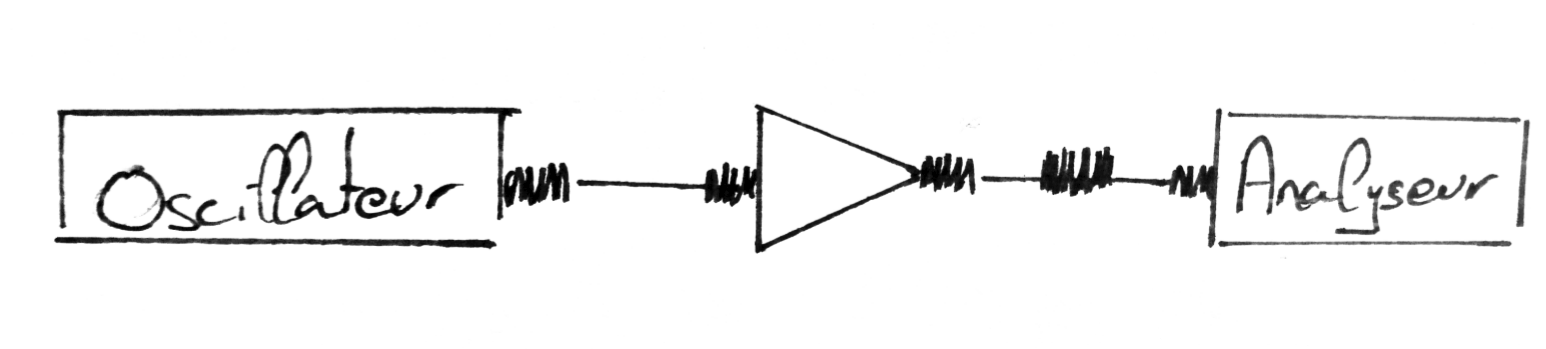
\includegraphics[scale = 0.25]{pic/montage.png}\\ \end{center}

En faisant varier la fréquence par pas de 50MHz, et en couvrant une plage allant de 100MHz à 1150MHz, 
nous relevons pour chaque cas la puissance de sortis, auquel nous additionons les pertes. Voici le graphique
que nous trouvons.

\begin{center}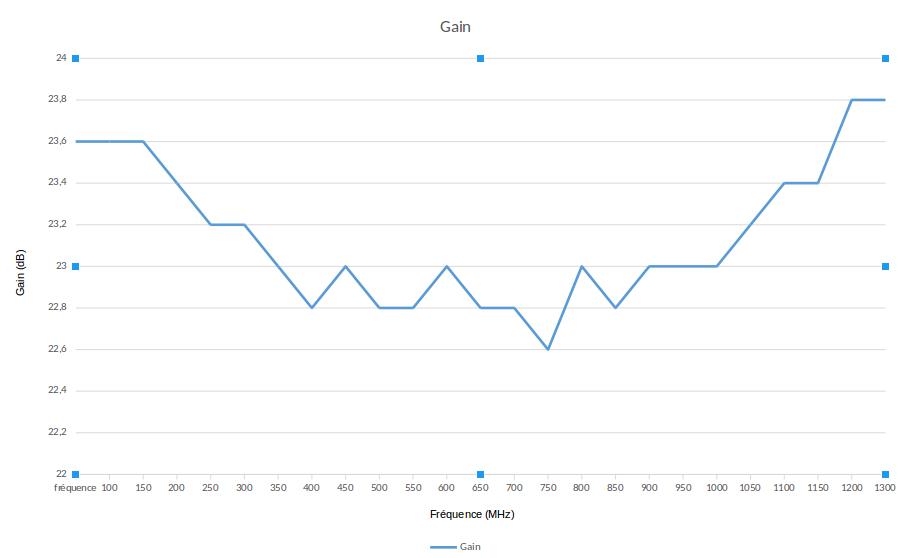
\includegraphics[scale = 0.4]{pic/gain_frequence.png}\\ \end{center}

Nous pouvons constater que le gain ce cet amplificateur varie entre 22.6 et 23.4 dB, selon la
fréquence d'entré. 

Maintenant que nous avons trouvé son amplification, nous pouvons déterminer sa zone de fonctionnement.

\chapter{Puissance}
\addcontentsline{toc}{chapter}{Puissance}

\section{Mesure de puissance}

Afin de déterminer l'IP3 ainsi que le point de compression, nous devons mesurer la puissance de
sortie en fonction de la puissance d'entré. Nous nous attendons à trouver une droite de pente 1
mais arrivera une certaine puissance à laquelle l'amplificateurne pourra plus amplifier correctement 
et la courbe deviendra plate. Le montage utilisé est le même que précédemment à la différence près
que la fréquence de l'oscillateur ne variera pas et sera fixé à 200MHz.

Voici la courbe obtenue :

\begin{center}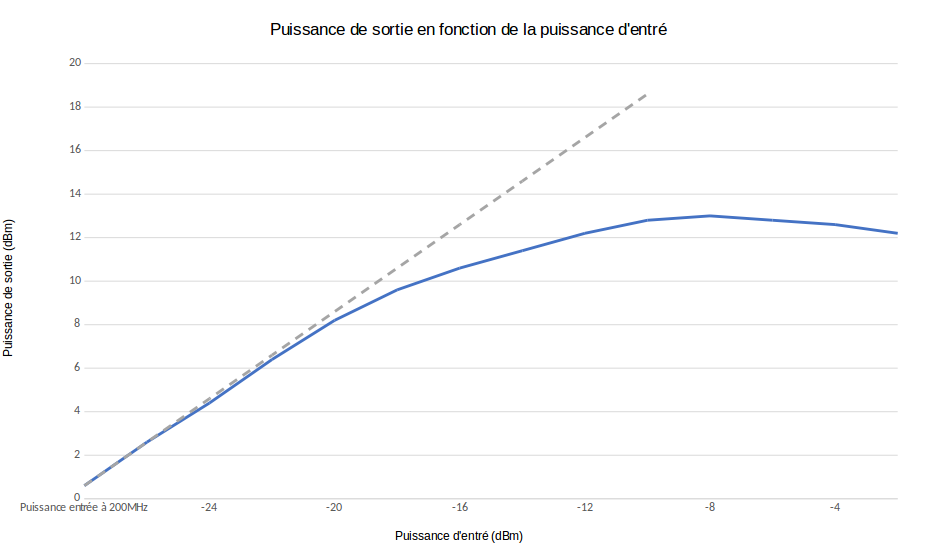
\includegraphics[scale = 0.4]{pic/puissance_graph.png}\\ \end{center}
    
Nous pouvons voir très clairement avec cette courbe que, progressivement, l'amplificateur perd sa linéarité
(courbe bleue) lorsqu'on la compare à l'amplification idéale (courbe en pointillé).
Nous utiliserons cette courbe afin de déterminer le point de compression à 1dB ainsi que le point d'IP3.

\newpage

\section{Point de compression}

Le point de compression représente la puissance (généralement celle de sortie) à laquelle l'amplificateur
aura perdu 1dB, la où il aurait du normalement en gagner un. C'est donc le point à partir duquel l'amplificateur 
aura perdu toute son amplification.
Nous pouvons le voir très facilement sur le graphique, et l'aproximer à une puissance de sortie d'environ 10dBm.
Les resulats de notre manipulation nous montre qu'il sagit d'une puissance de 9.6dBm

\section{IP3}

Le point d'IP3 représente le moment où les intermodulation d'ordre 3 coupe la droite d'amplification idéale comme
le montre la représentation ci-dessous :

\begin{center}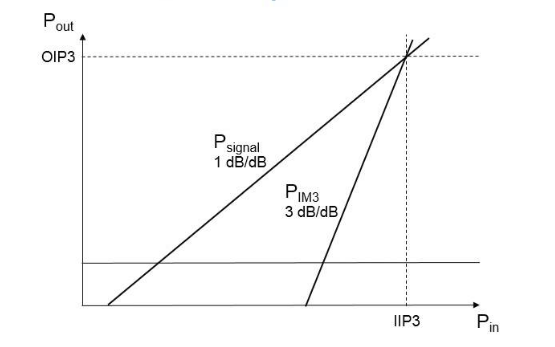
\includegraphics[scale = 0.4]{pic/IP3_exemple.png}\\ \end{center}

Pour cela, nous allons utiliser un coupleur, afin de faire entrer dans notre amplificateur deux fréquences différentes.
Ces deux fréquences devront être légérement décaler sans quoi nous verions une oscillation sur le signal de sortis.
Ainsi, nous pourrons calculer l'IP3 grâce à une formule sous deux condition :
\begin{itemize}
    \item Les deux fréquences d'entrée doivent être à la amplitude
    \item L'IM3 doit être inférieur à 40dBc 
\end{itemize}
Voici la formule que nous allons utiliser : $ \mbox{IP3}=P_{1^{er}ton} + \frac{\mbox{\itshape{IMD3}}}{2}$.\\
Voici alors le montage que nous allons utiliser :

\begin{center}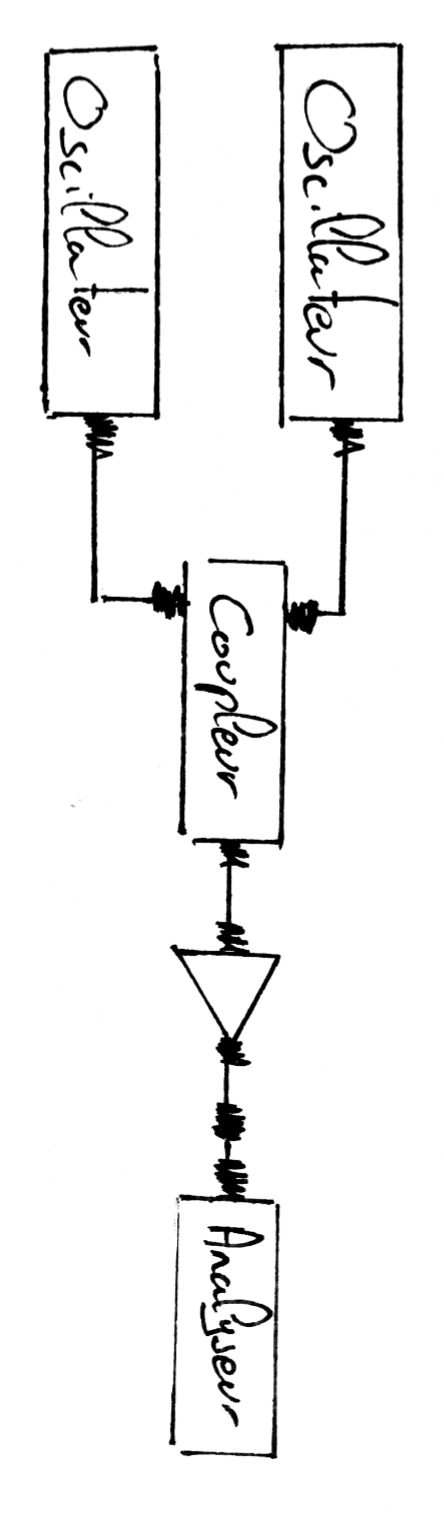
\includegraphics[scale = 0.2, angle =90]{pic/IP3_montage.png}\\ \end{center}

    
Nous avons ensuite pu extraire la puissance des différentes harmonique 2 et 3 dont voici le graphique :

\begin{center}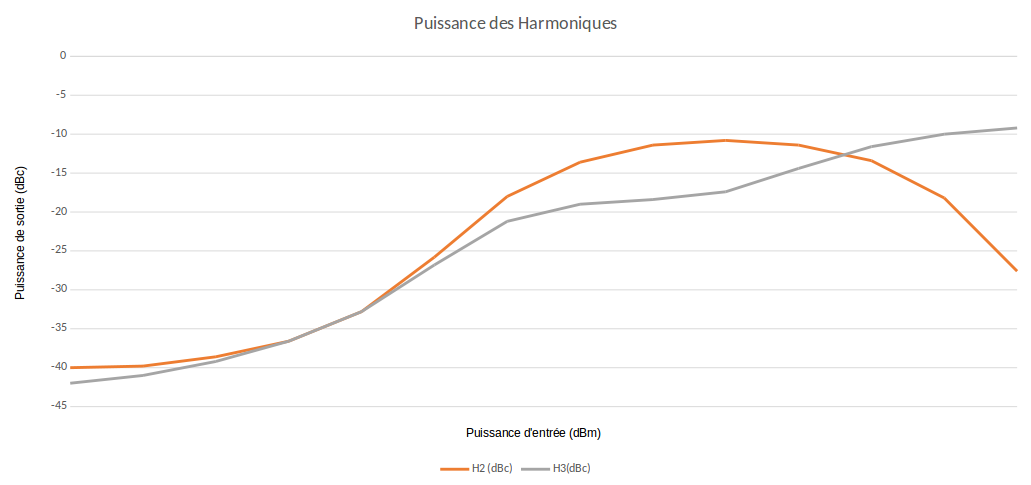
\includegraphics[scale = 0.4]{pic/harmonique_graph.png}\\ \end{center}

Voici les données que nous obtenons :
\begin{itemize}
    \item $P_{1^{er}ton} = -4.4dBm = 1.6dBm$ en prenant en compte les pertes.
    \item $P_{IM3} = -46.2dBm = 41.8dBc$
\end{itemize}

Nous pouvons alors faire le calcul de l'IP3 : 

$$IP3 = 1.6 + \frac{41.8}{2} = 22.5dBm $$

Il est à noté que plus cette valeur est haute, de meilleur qualité est l'amplificateur, son IM3
grandissant peu au fur et à mesure que sa puissance d'entré augmente.

\chapter{Analyseur de réseaux}
\addcontentsline{toc}{chapter}{Analyseur de réseaux}




\chapter{Conclusion}
\addcontentsline{toc}{chapter}{Conclusion}










\end{document}